%% Header, styling stuff
\documentclass[11pt]{article}
\setlength{\topmargin}{-.5in}
\setlength{\textheight}{9in}
\setlength{\oddsidemargin}{.125in}
\setlength{\textwidth}{6.25in}
\usepackage{graphicx}

\begin{document}

%%----------------
%% Title
%%----------------
\title{Sirius Detailed Design}
\author{Platform \& APIs Team}
\maketitle

This document is intended document Sirius’ design, so future developers can understand the system at a reasonable level, and so that we can record important design decisions somewhere in prose.  

%%----------------------
%% Theory of Operation
%%----------------------
\section{Theory of Operation}
TBD


%%---------------------
%% Design Overview
%%---------------------
\section{Design Overview}
\subsection{Sirius Interface}

\subsection{Actor Hierarchy}
\scalebox{0.7}{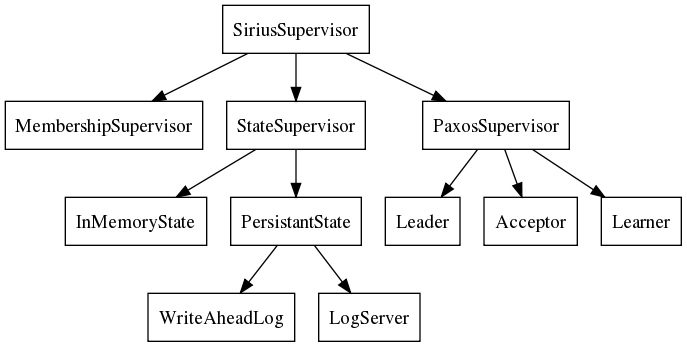
\includegraphics{img/actor_hierarchy.png}}

\subsubsection{Sirius Supervisor}

\subsection{Initialization}

%%-------------------------
%% Write Ahead Log Format
%%-------------------------
\section{Write Ahead Log Format}

%%------------------------------
%% Write Ahead Log Format:
%%    Principles of Some Import
%%------------------------------
\subsection{Principles of Some Import}
The Sirius write-ahead log is designed with the following principles in mind, in rough priority order:

\begin{itemize}
\item It must be possible to reconstruct the entire state of a system built on top of Sirius by replaying the write-ahead log.
\item The write-ahead log should be easily compactable, so it can serve as our persistent storage format for the state of a system built on Sirius, rather than using a separate snapshot mechanism.
\item The log should be as human readable as it can be, or, readability by a human is more important than squeezing as much information into a given number of bytes as possible.
\end{itemize}


%%------------------------------
%% Write Ahead Log Format:
%%    Design Overview
%%------------------------------
\subsection{Design Overview}

The log file is plain text, UTF-8 encoded.  Each entry begins with a checksum, and is terminated by a line feed (LF/'\textbackslash n'/U+000A). The checksum covers all data from the byte after the checksum to the line feed, inclusive.

Fields in an individual log entry are pipe (U+007C) delineated. Pipe characters and all whitespace\footnote{See http://docs.oracle.com/javase/6/docs/api/java/lang/Character.html\#isWhitespace(char)} are disallowed as parts of the log elements.  For convenience, a pipe character is placed immediately after the checksum.

An typical log entry would look something like:
\begin{center}
\em Checksum\textbar Action Type\textbar Key\textbar Sequence\textbar Timestamp\textbar Payload\textbackslash n
\end{center}


%%------------------------------
%% Write Ahead Log Format:
%%    Field Definitions
%%------------------------------
\subsection{Field Definitions}

\subsubsection{Checksum}
Hex encoded FNV-1a\footnote{See http://en.wikipedia.org/wiki/Fowler\%E2\%80\%93Noll\%E2\%80\%93Vo\_hash\_function} hash of the byte array that represents the rest of the log entry, including the pipes and terminating new line.

\subsubsection{Action Type}
A String that represents the type of action to take for a given log entry.  For the most part, these will mirror HTTP semantics.

\begin{center}
\begin{tabular}{|l|p{3.5in}|}
\hline
\multicolumn{2}{|c|}{Action  Types}\\ \hline
\textbf{PUT} & An HTTP PUT\\ \hline
\textbf{DELETE} & An HTTP DELETE\\ \hline
\textbf{CONDITIONAL\_PUT} & A conditional HTTP PUT, which may or may not have succeeded.   Since the log is write-ahead, we won’t know if the PUT will be successful at log writing time.\\ \hline
\textbf{CONDITIONAL\_DELETE} & Same as above, but for HTTP DELETE.\\ \hline
\textbf{COMPACTION\_HINT} & A hint that tells the compaction algorithm whether a particular conditional put or delete that comes earlier in the log was successful.\\ \hline
\end{tabular}
\end{center}

\subsubsection{Key}
A key that’s used to determine what sort of action should be taken.  This is going to be something like a partial URL, so something like /videos/1234.

For instance, a PUT to a key of /videos/1234 might add a video represented by the payload to a map, along with adding it to some secondary indices.  

Note that pipes and various whitespace are not allowed in the key, though they may be allowed in URIs.

\subsubsection{Sequence}
Strictly increasing sequence number that defines a total order of requests in the log, across all nodes in the system.  This is a String representation of a twos-complement \textbf{signed}\footnote{Because Java that’s why.} 64 bit integer, and must not fall outside the range representable in that scheme.

\subsubsection{Timestamp}
UTC timestamp in some ISO 8601 compliant format.

\subsubsection{Payload}
Base64 encoded binary payload for the log entry.  This is probably some representation of the data needed to do a PUT to a given resource.


%%------------------------------
%% Write Ahead Log Format:
%%    Compaction Algorithm
%%------------------------------
\subsection{Compaction Algorithm}

The log file will increase in size indefinitely with time so we  need to be able to apply certain techniques to compact the number of entries that make up a log file. Compacting the raw log file means that for the same entry in the log file, identified by its unique entry key, we should be able to persist the most recent entry and discard the previous entries from the log file. This applies to both event types: PUT and DELETE. By doing this, the size of the log file will be manageble and we also reduce the time it takes to reconstruct the machine state from the log file.

The current implementation compacts the log file by reading all each line in the log file and storing it in a HashMap where the key is the entry key and the value is the actual entry. Processing all lines in the log file means that we and up with a HashMap that has a unique key set of all the entries in the log file and the most recent entry as its value. We convert the HashMap into a List of entries and we sort it by entry sequence number, just to make sure that the new compacted version of the log file is ordered. The final output of this process is an ordered List of unique log entries. If you replay this compacted log, you should be able to construct the same exact state as if we were to replay the raw log.

%%------------------------------
%% Cluster Membership:
%%    Join Algorithm
%%------------------------------
\section{Cluster Membership}
Cluster membership is maintained by the membership subsystem.  It is this subsystems responsibility for maintaining the Set of all members in the cluster.  This membership is stored in a shared area and is accessible to all local subsystems.  It is an unwritten rule that only the membership subsystem is allowed to modify membership.

\subsection{Implementation}
Membership is stored in a file which is polled by the membership subsystem. This file contains the Actor Address\footnote{http://doc.akka.io/docs/akka/snapshot/general/addressing.html} of each of the cluster members on new lines.

\end{document}
